\chapter{Анализ предметной области}
\section{Современное состояние контейнеризации и роль реестров образов}

Контейнеризация стала фундаментальной технологией современной IT-индустрии, кардинально изменившей подходы к разработке, поставке и эксплуатации программного обеспечения. Согласно исследованиям, более 70\% организаций используют контейнеры в среде разработки крупных сервисов, причем рост адаптации составляет порядка 20\% в год \cite{slashdata2024}. Стремительный рост обусловлен преимуществами, которые предоставляют контейнерные технологии: изоляция приложений, переносимость, эффективное использование ресурсов и ускорение процессов развертывания.

На рисунке~\ref{fig:usage} представлена диаграмма использования контейнерых приложений крупными компаниями в 2024 году.

\begin{figure}[h!]
	\centering
	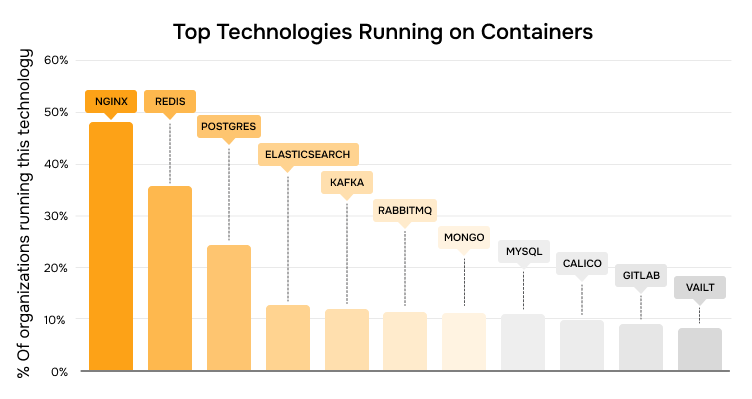
\includegraphics[width=0.8\textwidth]{usage}
	\caption{Диаграмма использования контейнерых приложений крупными компаниями в 2024 году}
	\label{fig:usage}
\end{figure}

Технология Docker стала стандартом в области контейнеризации \cite{mill2020} -- она предоставила разработчикам простой и унифицированный интерфейс упаковки приложений со всеми зависимостями, что решило проблему совместимости на всех этапах жизненного цикла ПО.

В микросервисной архитектуре, которая доминирует в современных облачных приложениях, количество контейнерных образов может достигать тысяч и десятков тысяч. Каждый сервис, каждая его версия требуют отдельного образа. Управление этим множеством артефактов становится критически важной задачей, сравнимой по сложности с управлением исходным кодом \cite{gartner2023}.

Роль реестров контейнерных образов в этой экосистеме невозможно переоценить. Реестры выполняют функции, аналогичные репозиториям исходного кода, но для бинарных артефактов. Они обеспечивают:

\begin{enumerate}
		\item централизованное хранение -- единый источник данных для всех контейнерных образов организации;
	\item версионирование и контроль изменений -- возможность отслеживать историю изменений образов;
	\item распределение артефактов -- эффективную доставку образов до сред выполнения;
	\item контроль доступа -- разграничение прав на чтение и запись различных категорий пользователей.
\end{enumerate}

Особую значимость реестры образов приобретают в контексте DevOps практик и процессов непрерывной интеграции и доставки (CI/CD). Современные CI/CD пайплайны генерируют десятки и сотни новых версий образов ежедневно, и без надежной системы управления этими артефактами эффективная работа становится невозможной \cite{luksha2020}.

Проблема безопасности цепочки поставок ПО также выдвигает дополнительные требования к системам управления реестрами. После ряда громких инцидентов, связанных с компрометацией контейнерных образов, организации осознали необходимость внедрения строгого контроля целостности, сканирования уязвимостей и цифровой подписи образов \cite{sysdig2024}.

Рынок систем управления реестрами демонстрирует активный рост. Согласно анализу, ежегодный прирост рынка составляет около 25\%, причем наибольшую динамику показывают решения с открытым исходным кодом, которые сочетают в себе корпоративный функционал и гибкость развертывания \cite{forrester2022}.

Таким образом, системы управления реестрами контейнерных образов превратились из простых хранилищ в сложные платформы, обеспечивающие безопасность, наблюдаемость и управляемость всего жизненного цикла контейнерных артефактов. Их роль в современных ИТ-ландшафтах продолжает усиливаться по мере роста масштабов использования контейнерных технологий.


\section{Понятия Docker и технологии контейнеризации}
\subsection{Основы контейнеризации и Docker}

Контейнеризация представляет собой технологию изоляции приложений на уровне операционной системы, позволяющую запускать процессы в изолированных пользовательских пространствах (контейнерах), разделяющих ядро хостовой системы. В основе современных технологий контейнеризации лежит концепция docker-образа - неизменяемого шаблона, состоящего из слоев, доступных только для чтения, каждый из которых описывает определенное изменение файловой системы \cite{mill2020}. Эти слои обеспечивают эффективное хранение и распространение приложений, поскольку общие слои могут использоваться несколькими образами. Для внесения изменений создаются собственные надстройки, которые записываются в самый верхний слой, который доступен для записи:

Docker-контейнер представляет собой запущенный экземпляр образа, изолированный от других контейнеров и хост-системы \cite{docker-spec}. Изоляция достигается за счет использования возможностей ядра Linux, таких как namespaces и cgroups. Важным свойством контейнеров является их переносимость: образ, собранный на одной системе, будет идентично работать на любой другой системе с поддержкой Docker.

На рисунке~\ref{fig:docker-layers} представлена структура Docker-образа.	

\begin{figure}[h!]
	\centering
	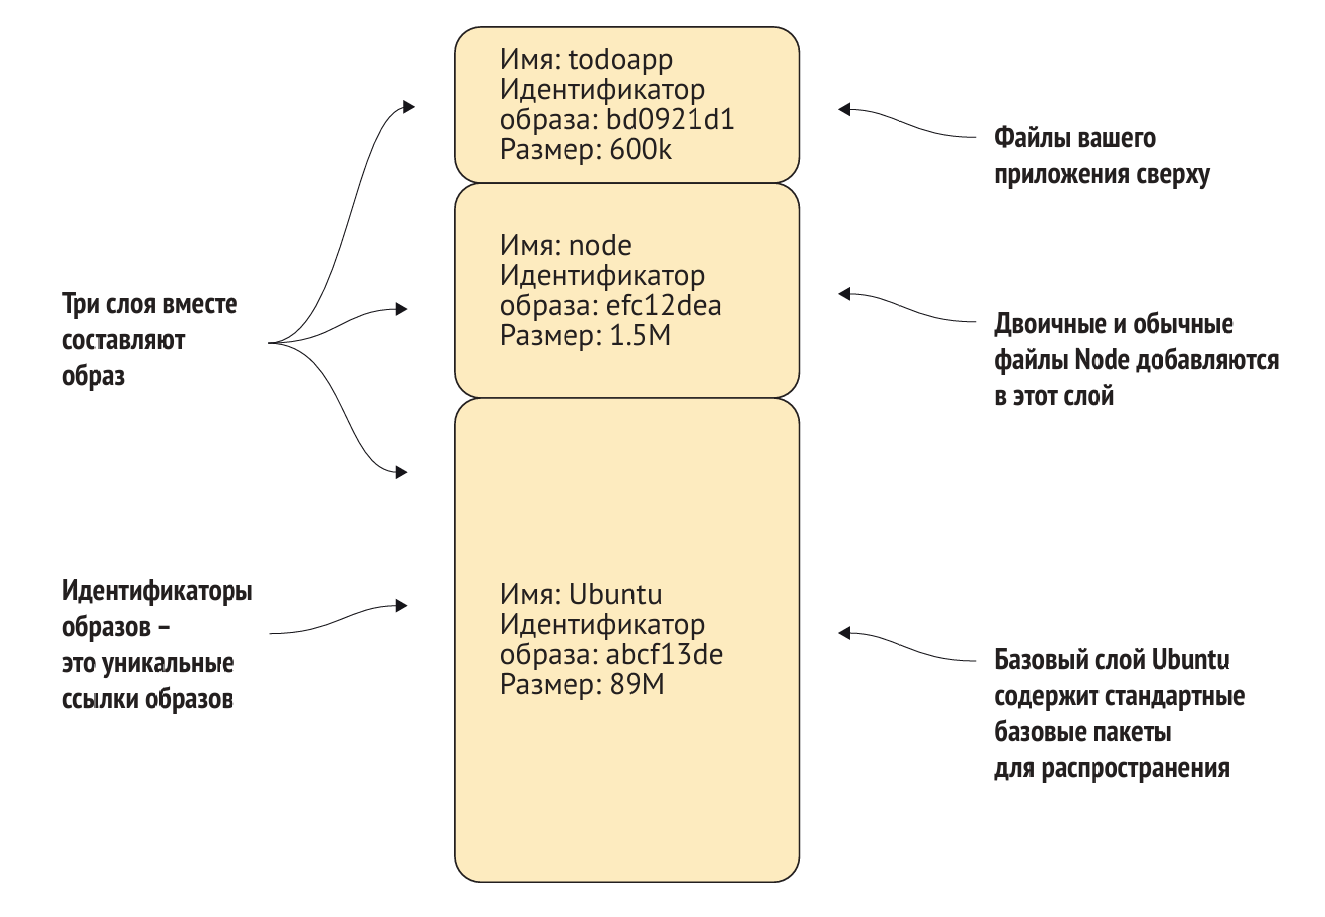
\includegraphics[width=0.8\textwidth]{layers}
	\caption{Структура Docker-образа: базовый образ, слои приложений и контейнерный слой}
	\label{fig:docker-layers}
\end{figure}

\subsection{Реестры контейнерных образов и их компоненты}
Системы управления реестрами образуют центральный элемент инфраструктуры контейнеризации. Реестр Docker-образов функционирует как специализированное хранилище, предоставляющее REST API для операций загрузки и скачивания образов \cite{docker-spec}. Внутри реестра образы организованы в репозитории - логические группы, обычно соответствующие отдельным приложениям или сервисам.

Каждый репозиторий содержит одну или несколько версий образа, идентифицируемых с помощью тегов. Тегирование позволяет управлять версиями артефактов и обеспечивает гибкость в развертывании приложений \cite{harbor-docs}. Помимо Docker-образов, современные реестры поддерживают хранение различных типов артефактов. К таким артефактам относятся, например, Helm-чарты -- пакеты, описывающие набор ресурсов Kubernetes для развёртывания приложений, а также любые OCI-совместимые (Open Container Initiative) объекты, соответствующие открытому стандарту формата контейнеров и артефактов. Эта возможность превращает реестр из узкоспециализированного хранилища в универсальную платформу для управления бинарными артефактами \cite{cncf2022}.

\subsection{Безопасность и управление в реестрах}
В контексте корпоративного использования реестры образов должны обеспечивать комплексные механизмы безопасности. Управление доступом на основе ролей (RBAC) позволяет гибко настраивать политики доступа для различных категорий пользователей. Интеграция с корпоративными системами аутентификации, такими как LDAP (Lightweight Directory Access Protocol) — протокол для доступа к службам каталогов, и OIDC (OpenID Connect) — современный протокол аутентификации поверх OAuth 2.0, обеспечивает единое (централизованное) управление учетными записями и соответствие корпоративным стандартам безопасности.

Сканирование уязвимостей стало неотъемлемой функцией современных реестров. Этот процесс предполагает автоматический анализ компонентов образа на наличие известных уязвимостей и предоставление отчетов о безопасности \cite{sysdig2024}. Для обеспечения целостности и доверия к артефактам применяется цифровая подпись образов, гарантирующая их подлинность и неизменность.

Репликация между экземплярами реестра обеспечивает отказоустойчивость и географическое распределение, что особенно важно для организаций с распределенной инфраструктурой \cite{cilic2023}. Механизмы репликации могут быть синхронными или асинхронными, в зависимости от требований к согласованности данных и задержкам.

\subsection{Стандарты и спецификации}
Развитие экосистемы контейнеризации привело к появлению стандартов, обеспечивающих совместимость между различными инструментами. Спецификация OCI (Open Container Initiative) определяет стандартные форматы контейнерных образов и сред выполнения \cite{oci-spec}. Этот стандарт обеспечивает переносимость образов, созданных с помощью Docker, в другие OCI-совместимые системы контейнеризации (Podman, containerd), способствуя интероперабельности инструментов экосистемы.

API Docker Registry стал стандартом для базового взаимодействия с реестрами образов. Однако современные корпоративные решения, такие как Harbor, расширяют его возможности, добавляя функции, критически важные для организаций: управление доступом на основе ролей (RBAC), сканирование образов на уязвимости, георепликацию, управление политиками хранения и поддержку разнородных артефактов (Helm-чарты, OCI) \cite{harbor-docs}. Поддержка как базового стандарта, так и его расширений обеспечивает интероперабельность между различными инструментами экосистемы контейнеризации, такими как оркестраторы (Kubernetes), системы CI/CD (Jenkins, GitLab CI) и сканеры безопасности (Trivy, Clair).

\section{Классификация задач управления реестром контейнерных образов}
\subsection{Задачи безопасности и соответствия требованиям}

Безопасность является критически важным аспектом управления реестрами образов, особенно в свете участившихся инцидентов, связанных с цепочкой поставок ПО. Реальные атаки демонстрируют различные векторы угроз: внедрение вредоносного кода в базовые образы, компрометация учетных записей с правами на запись в реестр и использование уязвимостей в самих системах управления реестрами \cite{sysdig2024}.

Аутентификация и авторизация системы должны предоставлять гибкие механизмы управления доступом, включая интеграцию с корпоративными системами каталогов (LDAP, Active Directory) и поддержку стандартов OIDC, OAuth 2.0. Управление доступом на основе ролей (RBAC) позволяет точно настраивать права для различных категорий пользователей, что является одним из самых строгих критериев безопасности управления \cite{harbor-docs}.

На рисунке~\ref{fig:rbac} представлена схема стандртов ролевого подхода к управлению доступом.	

\begin{figure}[H]
	\centering
	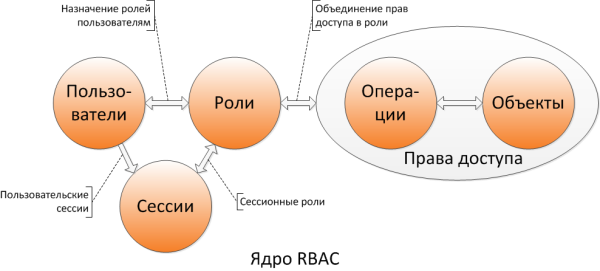
\includegraphics[width=0.5\textwidth]{rbac}
	\caption{Стандарты ролевого подхода к управлению доступом}
	\label{fig:rbac}
\end{figure}

Кроме этого, необходимо введение автоматического обнаружения известных уязвимостей в контейнерных образах стало обязательным требованием для корпоративных реестров \cite{aqua2023}. Современные системы интегрируют различные сканеры и предоставляют детальные отчеты о безопасности.

Цифровая подпись и проверка целостности необходимы для обеспечения доверия к артефактам. Для этого используются специализированные механизмы, как например Docker Content Trust -- встроенная в Docker Engine система, использующая набор ключей для подписи и проверки образов \cite{docker-spec}. Эта система применяют криптографические методы для создания цифровых подписей, что гарантирует, что образы не были изменены после их публикации и получены из доверенного источника.

\subsection{Задачи управления жизненным циклом артефактов}

Эффективное управление жизненным циклом контейнерных образов необходимо для поддержания порядка в реестре и оптимизации использования ресурсов. Системы должны предоставлять удобные механизмы для управления версиями образов через теги. Это включает поддержку семантического версионирования (Semantic Versioning, SemVer) — схемы, где номер версии структурированно указывает на характер изменений (мажорные, минорные, патчи), что помогает автоматизировать процессы обновления. Также необходима гибкая работа с тегами (метками), позволяющая, помимо версионных, использовать плавающие теги (latest, stable) и теги для различных сред (prod, staging)  \cite{docker-spec}.

Автоматическое удаление устаревших образов на основе настраиваемых правил помогает экономить дисковое пространство, что особенно актуально при больших объемах хранимых данных \cite{harbor-docs}. Установка лимитов на использование дискового пространства для проектов или пользователей предотвращает неконтролируемый рост объема данных и обеспечивает равномерное распределение ресурсов \cite{cilic2023}. Помимо Docker-образов, современные реестры должны поддерживать Helm-чарты, OPA-политики и другие OCI-артефакты, что делает их универсальными платформами для управления бинарными артефактами в облачной экосистеме \cite{cncf2022}.

\subsection{Задачи обеспечения доступности и производительности}

Для обеспечения бесперебойной работы систем, использующих реестр образов, необходимо решать комплекс задач, связанных с доступностью и производительностью.

Синхронизация данных между несколькими сущностями реестра обеспечивает отказоустойчивость и снижает задержки для распределенных команд, при этом репликация может быть синхронной или асинхронной в зависимости от требований к согласованности \cite{cilic2023}. Кэширование часто запрашиваемых образов ускоряет их получение и снижает нагрузку на внешние реестры, а проксирование запросов к публичным реестрам позволяет контролировать внешний трафик и обеспечивать дополнительный уровень безопасности \cite{harbor-docs}.

Возможность горизонтального масштабирования системы под растущую нагрузку является обязательным требованием для крупных организаций, что позволяет адаптироваться к увеличению числа пользователей и объема хранимых данных \cite{gartner2023}. Регулярное создание бэкапов метаданных и образов обеспечивает возможность быстрого восстановления после сбоев, минимизируя простои и потери данных в критических ситуациях \cite{sysdig2024}.

\subsection{Задачи интеграции и операционного управления}

Интеграция с существующей инфраструктурой и удобство операционного управления существенно влияют на успешность внедрения системы управления реестром. Поддержка webhook-ов и API для автоматизации процессов сборки и развертывания позволяет интегрировать реестр в процессы непрерывной интеграции и доставки, что ускоряет разработку и повышает ее надежность \cite{mill2020}.

Сбор метрик использования, логов операций и ведение аудиторского журнала обеспечивают возможность анализа работы системы и расследования инцидентов безопасности. Удобный веб-интерфейс для просмотра образов, управления правами доступа и анализа отчетов безопасности значительно упрощает ежедневную работу администраторов и разработчиков, снижая порог вхождения и уменьшая вероятность ошибок. Программные интерфейсы и инструменты командной строки предоставляют возможности для автоматизации задач управления и интеграции со скриптами, что позволяет создавать сложные сценарии работы с реестром и включать его в более крупные автоматизированные процессы.

\subsection{Система Harbor как эталонное решение}

Система Harbor представляет собой открытый реестр контейнерных образов корпоративного уровня, разрабатываемый под эгидой Cloud Native Computing Foundation (CNCF). Изначально созданный компанией VMware, Harbor быстро стал одним из наиболее популярных решений для управления артефактами в облачной экосистеме благодаря своей комплексной функциональности и активному сообществу contributors \cite{harbor-docs}. 

Архитектура Harbor построена вокруг модульной структуры, включающей основные компоненты: основные службы, отвечающие за базовые операции с образами, службы реестра, реализующие Docker Registry API, предоставляющий веб-интерфейс, дополнительные службы безопасности и тегирования для цифровой подписи образов \cite{harbor-docs}. Остальные службы предназначены для удобной интеграции с другими сервиса контейнеризации, согласно стандарту OCI. Такая архитектура обеспечивает гибкость развертывания и возможность масштабирования отдельных компонентов в зависимости от нагрузки.

На рисунке~\ref{fig:harbor} представлена архитектура системы управления реестром docker-образов Harbor.	

\begin{figure}[H]
	\centering
	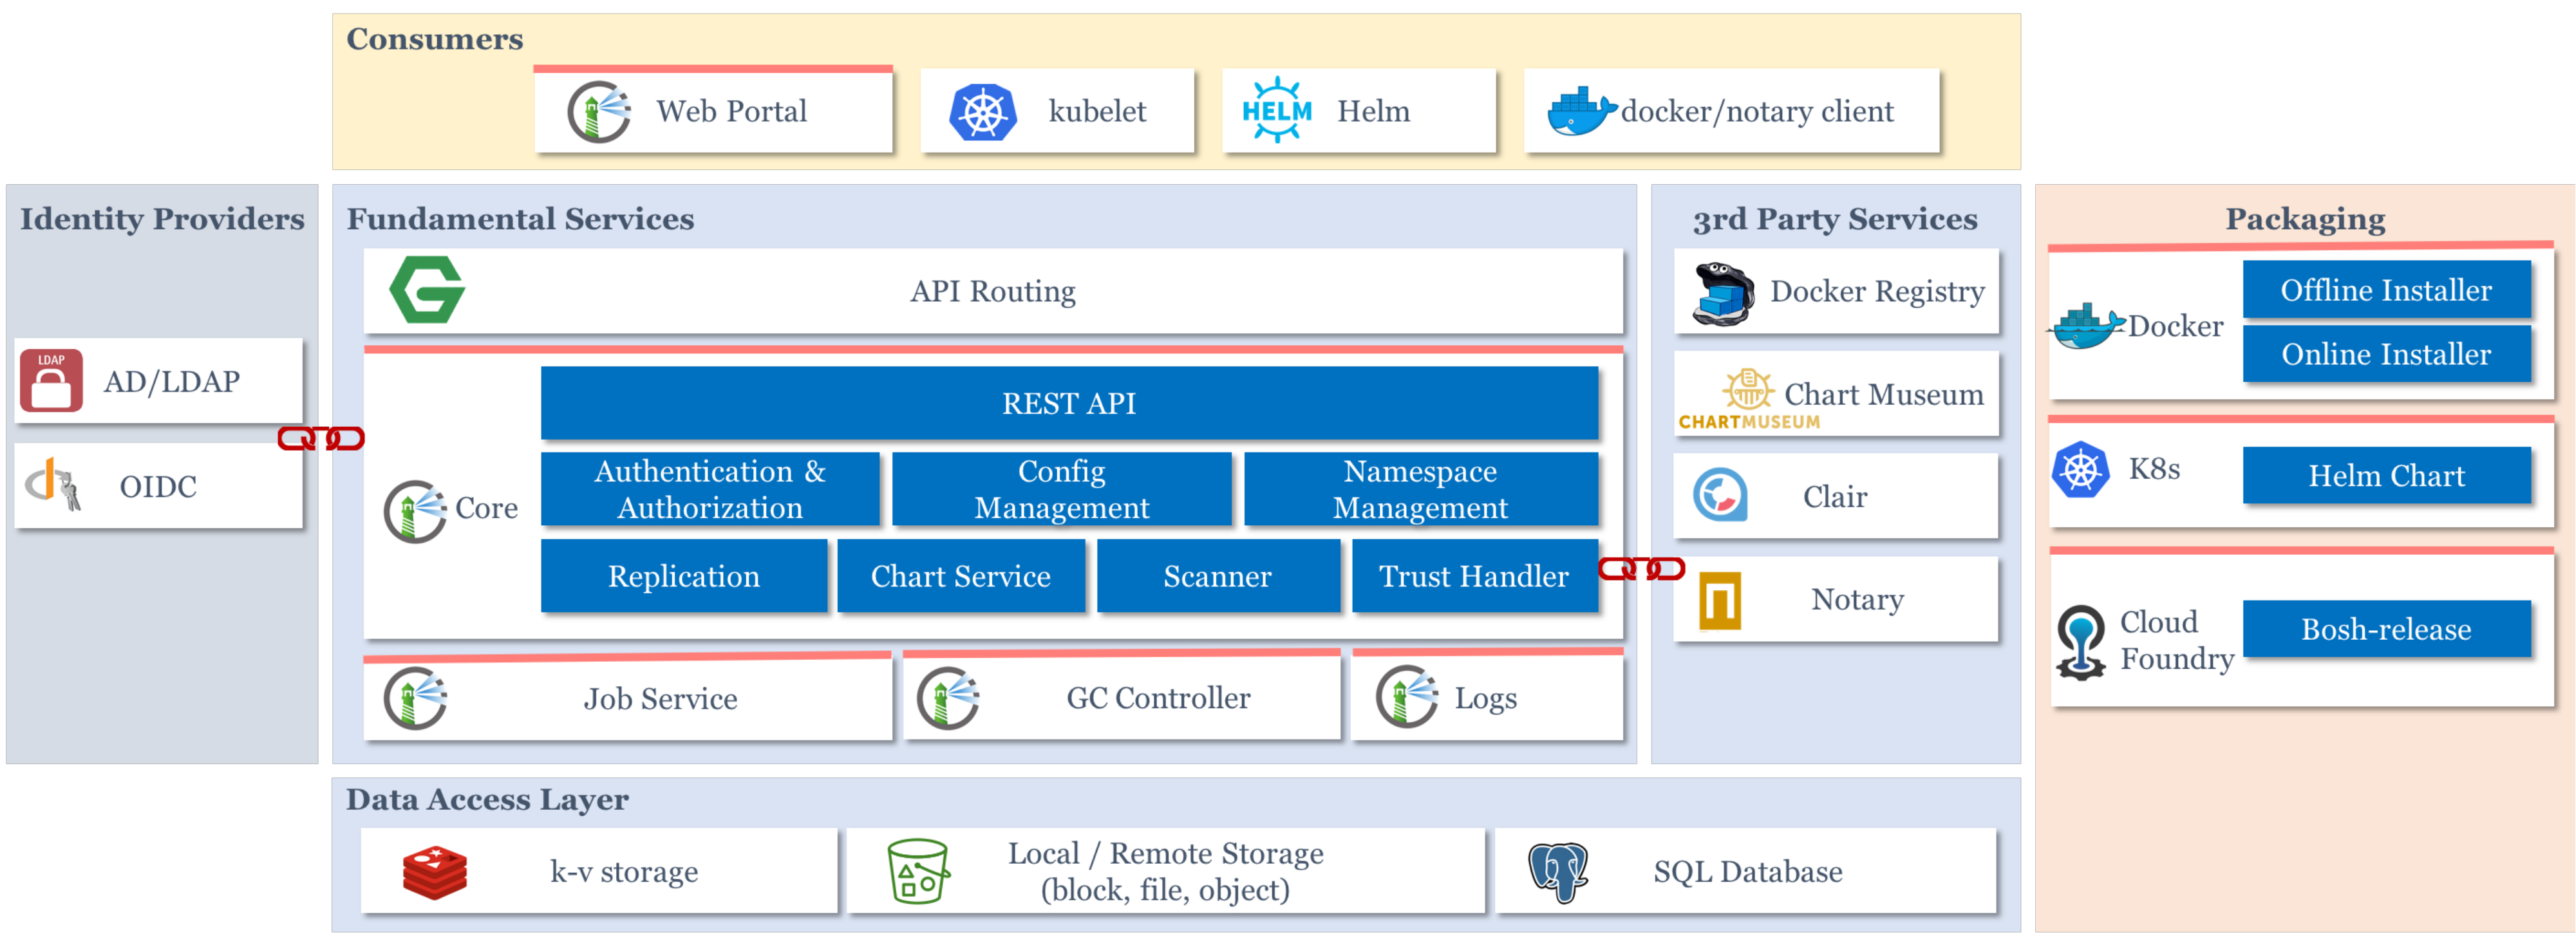
\includegraphics[width=0.9\textwidth]{harbor-architecture}
	\caption{Архитектура системы управления реестром docker-образов Harbor}
	\label{fig:harbor}
\end{figure}


Ключевой особенностью Harbor является встроенная поддержка механизмов безопасности, которые обычно требуют отдельной настройки в других решениях. Система включает интегрированное сканирование уязвимостей с использованием Clair, что позволяет автоматически анализировать образы на наличие известных уязвимостей сразу после их загрузки в реестр. Механизм цифровой подписи гарантирует целостность и аутентичность артефактов, предотвращая использование модифицированных образов в среде разработки \cite{harbor-docs}.

Управление доступом в Harbor реализовано через ролевую модель (RBAC) с возможностью интеграции с внешними системами аутентификации, включая LDAP, Active Directory и OIDC-провайдеры. Это позволяет крупным организациям использовать существующую инфраструктуру управления идентификацией и соблюдать корпоративные политики безопасности \cite{cilic2023}. Система поддерживает мультизадачность через проекты, где каждый проект может иметь собственные настройки доступа, политики хранения и квоты.

Функциональность репликации в Harbor обеспечивает синхронизацию образов между различными состояниями реестра, что критически важно для организаций с распределенной инфраструктурой. Поддержка как push, так и pull репликации позволяет гибко настраивать стратегии распределения артефактов между дата-центрами и облачными провайдерами \cite{cncf-landscape}. В сочетании с возможностями кэширования и проксирования внешних реестров это делает Harbor эффективным решением для построения распределенной системы управления артефактами.

Harbor также выделяется поддержкой различных типов артефактов помимо Docker-образов. Система может хранить Helm-чарты, OPA-политики и другие OCI-совместимые объекты, что превращает ее в универсальную платформу для управления всеми типами бинарных артефактов в cloud-native среде \cite{cncf2022}. Интеграция с популярными CI/CD системами через webhook-и и REST API обеспечивает seamless встраивание в процессы непрерывной интеграции и доставки.

Благодаря перечисленным характеристикам, Harbor является идеальным эталоном для сравнительного анализа систем управления реестрами. Его функциональность охватывает все ключевые аспекты, выделенные в предыдущих разделах: безопасность, управление жизненным циклом, обеспечение доступности и интеграционные возможности.


\clearpage

\section{Практическое развёртывание системы Harbor}

Для проверки функциональных возможностей, рассмотренных в предыдущих разделах, и для использования в качестве корпоративного реестра требуется корректное развёртывание системы Harbor. В данном подразделе представлен базовый порядок установки Harbor на операционную систему Ubuntu Server 22.04 LTS, который может быть адаптирован для других дистрибутивов Linux. Развёртывание описано в тестовом режиме; для производственной среды требуется дополнительная настройка, включая использование SSL-сертификатов, внешней базы данных и объектного хранилища \cite{harbor-docs}.


\begin{enumerate}
	\item аппаратные требования: минимум 4~ГБ ОЗУ, 2 ядра CPU, 40~ГБ дискового пространства для работы системы и хранения образов;
	\item программные зависимости: установленная ОС Ubuntu Server 22.04 LTS с обновлёнными пакетами;
	\item необходимое ПО: установка компонентов, которые являются зависимостями для Harbor:
	\begin{itemize}
		\item оболочка Docker Engine и Docker Compose;
		\item генератор OpenSSL.
	\end{itemize}
\end{enumerate}


Шаги установки следуют официальной документации проекта \cite{harbor-docs}.

\begin{enumerate}
	\item загрузка установщика: архив с установщиком Harbor загружается с официального GitHub-репозитория. Рекомендуется выбирать последнюю стабильную версию;
	
	\item настройка конфигурации: основные параметры системы задаются в файле `harbor.yml`. Минимальная конфигурация для тестового запуска включает:
	\begin{itemize}
		\item задание сетевого имени или IP-адреса хоста (`hostname`);
		\item настройка пароля для административного интерфейса (`harbor\_admin\_password`);
		\item отключение HTTPS для упрощения первой установки (комментарий для раздела `https:`, активация порта 80 в разделе `http:`).
	\end{itemize}
	
	\item запуск скрипта установки: выполнение подготовительного скрипта, который загружает необходимые образы контейнеров и генерирует конфигурации.
\end{enumerate}

В процессе работы скрипт проверит наличие зависимостей, загрузит образы контейнеров Harbor и запустит все службы через Docker Compose.


После успешного выполнения скрипта система будет доступна:
\begin{enumerate}
	\item через веб-интерфейс: по адресу \texttt{http://<IP\_СЕРВЕРА>}. Логин: \texttt{admin}, пароль: заданный в `harbor.yml`;
	\item через Docker CLI: для работы с реестром необходимо добавить его адрес в конфигурацию Docker (для тестовой установки без HTTPS).
\end{enumerat}

Данные шаги позволят полностью развернуть Harbor на операционной системе на основе UNIX.

В листингах~\ref{lst:download-harbor}--\ref{lst:docker-insecure} представлены основные команды для корректной установки и развёртывания Harbor.


\begin{lstlisting}[caption={Установка базовых зависимостей на Ubuntu Server.}, label={lst:install-deps}, language=bash, captionpos=b]
	sudo apt update && sudo apt upgrade -y
	sudo apt install -y docker.io docker-compose-v2 openssl
	sudo systemctl enable docker && sudo systemctl start docker
\end{lstlisting}

\begin{lstlisting}[caption={Загрузка и распаковка установщика Harbor.}, label={lst:download-harbor}, language=bash, captionpos=b]
	wget https://github.com/goharbor/harbor/releases/download/v2.10.0/harbor-online-installer-v2.10.0.tgz
	tar xzf harbor-online-installer-v2.10.0.tgz
	cd harbor
\end{lstlisting}

\begin{lstlisting}[caption={Настройка Docker для работы с небезопасным реестром (для теста).}, label={lst:docker-insecure}, language=bash, captionpos=b]
	echo '{"insecure-registries": ["<IP>"]}' | sudo tee /etc/docker/daemon.json
	sudo systemctl restart docker
\end{lstlisting}

Дальнейшие шаги по настройке интегрированного сканирования уязвимостей, репликации, подключения внешних систем аутентификации (LDAP/OIDC) и настройки политик хранения выполняются через веб-интерфейс или путём редактирования конфигурационных файлов, что подтверждает гибкость и готовность Harbor к использованию в корпоративной среде \cite{cncf-landscape}.

\clearpage